%% Methodology
%%=========================================

\chapter{Methodology}
\label{ch:methodology}
This chapter presents the research methodology that was used in the process of writing this thesis. Section \ref{sec:research_questions_and_approach} looks closer at the research questions which we defined in the previous chapter. Section \ref{sec:research_approaches} presents the research approach, and Section \ref{sec:research_strategy} presents our choice of research strategies. In Section \ref{sec:data_generation_methods_and_data_analysis} we present our data generation methods and how we did our data analysis .

%%=========================================

\section{Evaluating Research Questions}
\label{sec:research_questions_and_approach}
We have already presented our research questions as:

\begin{description}
    \item[Research Question 1]{\textit{Does ambiguity in character signature sequences impact recognition rates?}}
    \item[Research Question 2]{\textit{Can a signature sequence based model handle multiple fonts at the same time?}}
    \item[Research Question 3]{\textit{Is a signature sequence based model unable to handle noise?}}
\end{description}

\newpage
In this section we will look closer at how we may give an answer to these questions in a meaningful way:

\begin{description}
    \item[RQ1:]{We knew ambiguity could be a problem due to how signatures of different letters may be identical. This was made clear early in testing and is explained further in Section \ref{sec:ambiguous_input}. To answer this research question we would need to conduct tests and experiments to see how ambiguity affected the recognition rates.}
    \item[RQ2:]{Recognizing words with a single font is one problem, but combining two or more fonts poses more complex problem, especially given the nature of the problem. This research question could, similarly to \textbf{RQ1}, be answered by running tests with text written in multiple fonts and see how the recognition rates were affected. Sections \ref{sec:tuning_input_data}, \ref{sec:use_of_fonts}, and \ref{sec:other_factors} explains how the typography of fonts may affect recognition.}
    \item[RQ3:]{While clean and well-formatted data is preferable, we may not always be so lucky that our data is completely noise free. Noise-induced data is also much more ``realistic", in a real world perspective, than 100\% perfect data. Investigating how well a model can handle certain degrees of noise is interesting, as it could say something about how robust it is. Investigating this could be done by running tests and introduce noise increasingly until the recognition rates deteriorate beyond a certain point.}
\end{description}

%%=========================================

\section{Research Approaches}
\label{sec:research_approaches}
We chose to follow the research process presented by \citep{oates2005researching}. Figure \ref{fig:model_research_process} gives an overview of their research process and its components. The overview illustrates how different research approaches can be formed by mixing and matching various types of strategies, data generation methods, and types of data analysis.

\begin{figure}[ht]
    \centering
    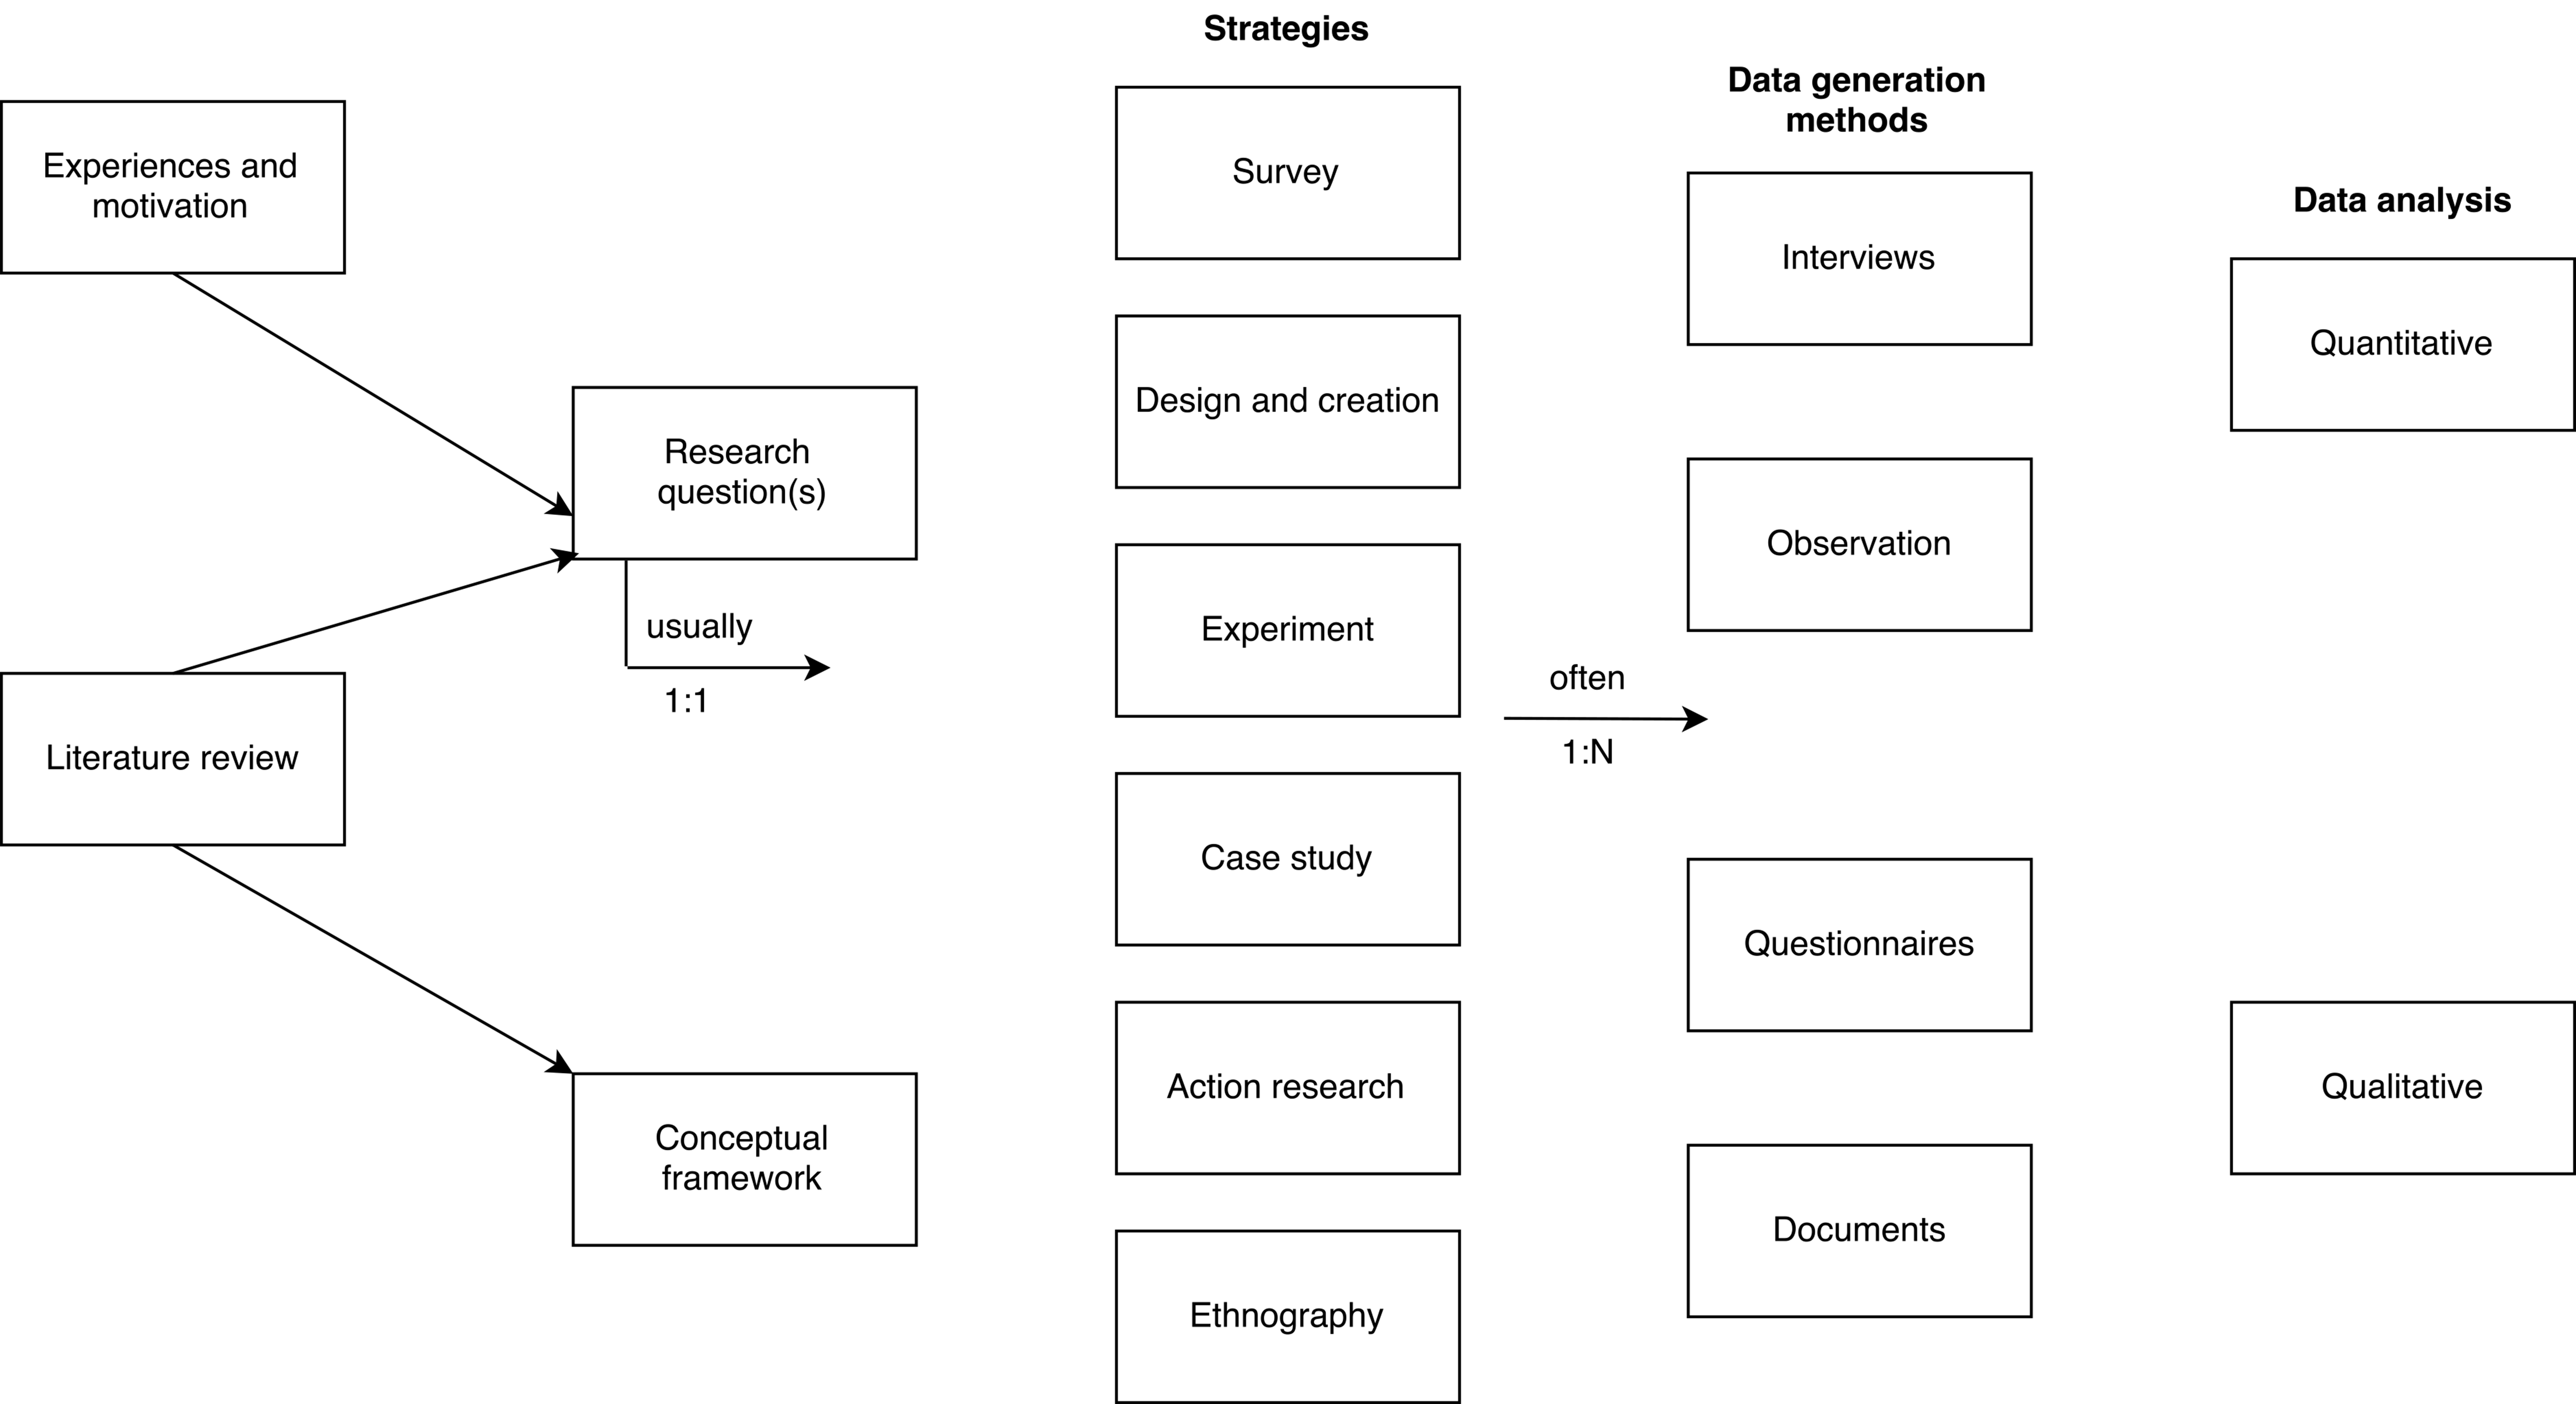
\includegraphics[width=1\textwidth]{fig/methodology/research_strategies.png}
    \caption{Model of the research process}
    \label{fig:model_research_process}
\end{figure}

Our literature review is presented in Chapter \ref{ch:related_work}. The research questions was presented in Section \ref{sec:goals_and_research_questions}, and was explained further in Section \ref{sec:research_questions_and_approach}. The conceptual framework is what is presented throughout this chapter. Our choice of research strategy is presented in Section \ref{sec:research_strategy}, and our choice of data generation methods, as well as our data analysis approach, is presented in Section \ref{sec:data_generation_methods_and_data_analysis}.

%%=========================================

\section{Research Strategy}
\label{sec:research_strategy}
The research strategy used in this thesis was carefully chosen on the basis of what our research questions and overarching goal was, and how they could best be answered. We argued that the research questions, as well as the research goal, could best be answered by conducting experiments and tests. 

We decided to use the research strategy of design and creation combined with the research strategy of experiments for the work conducted in this thesis. \citep{oates2005researching} states that is is most common to use a single research strategy, but that it is also possible to combine one or more. Our combination of research strategies allowed us to iteratively build one or more models, and to test various approaches to find optimal solutions. We followed the strategy of design and creation for the most part, but relied on experiments to move forward in the process. We also used experiments to answer the research questions, which would be the most important part of the research. While the strategy of design and creation is built on the concept of iteratively building a product, experiments is a strategy that investigates cause and effect relationships. They can be used together to help steer the process in the right direction during the development and exploration stages.

\subsection{Design and Creation}
\label{sec:design_and_creation}
Development of a new IT product is the main focus of the design and creation research strategy. IT products are also called artefacts, and there are four of these \citep{march1995design, oates2005researching}:

\begin{itemize}
    \item\textbf{Constructs:} the concepts or vocabulary used in a particular IT-related domain. For example, notions of entities, objects or data flows.
    \item\textbf{Models:} combinations of constructs that represent a situation and are used to aid problem understanding and solution development. For example, a data flow diagram, a use case scenario or a storyboard.
    \item\textbf{Methods:} guidance on the models to be produced and process stages to be followed to solve problems using IT. For example, formal, mathematical algorithms, or commercialized and published methodologies.
    \item\textbf{Instantiantions:} a working system that demonstrates that constructs, models, methods, ideas, genres or theories can be implemented in a computer-based system.
\end{itemize}

In our case, the artefact we want to develop during our research would fall into the category of instantiantions. This artefact would be a fully functional system that would answer both our research goal, as well as our research questions.  As this system would be an essential part of the research process, it would be important that it can could considered as research, and not just as a demonstration of technical powers. It was therefore crucial that the system was not only developed, but that the process also assert the academical qualities, such as analysis, explanation, argument, justification, and critical evaluation \citep{oates2005researching}. This meant that every part of our system, and the process of building it, would need to be explained and reasoned.

\subsubsection{Approach}
\label{methodology-design-and-creation-approach}
The approach in design and creation revolves around a problem-solving strategy. It utilizes an iterative process over five steps \citep{vaishnavi2004design, oates2005researching}:

\begin{itemize}
    \item\textbf{Awareness:} involves recognizing a problem. This step is necessary to find what problem we are trying to solve.
    \item\textbf{Suggestion:} is the step where we create a tentative idea of how the problem might be addressed.
    \item\textbf{Development:} is where we implement ad idea from the previous step.
    \item\textbf{Evaluation:} involves examine the artefact and evaluations are done to estimate its worth and deviations from the expectations.
    \item\textbf{Conclusion:} is the final step in the cycle where results are collected and written down. Gained knowledge is identified and any unexpected or unexplainable results could lay the ground for further research.
\end{itemize}

It is important to understand that these steps are not necessarily followed in a strict manner. Instead, they work as guidelines, and the process is more of a fluid iterative cycle where the approach may shift depending on problem or situation. \citep{oates2005researching} explains how these cycles work and what you as a researcher achieves by using this research method as follows:

\begin{quote}
    Thinking about a suggested tentative solution leads to greater awareness of the nature of the problem; development of a design idea leads to increased understating of the problem and new, alternative tentative solution; discovering that a design doesn't work according to the researcher's expectations leads to new insights and theories about the nature of the problem, and so on. 
\end{quote}

The goal is to work out a prototype that is gradually modified until a satisfactory implementation is produced. One of the biggest advantages of this approach is that it is not necessary to fully understand a problem before developing prototypes and exploring tentative solutions. This research strategy also opens up the possibilities of testing prototypes often and comparing results along the way to see if one direction or approach works better than others. As an essential part of this strategy, it must be made clear how the implemented solution emerged as a result of the repeated cycles. Without a thought-through design rationale, the final implementation may appear to be the result of a hacked together solution without any recollection of the trial and error phase.

\subsection{Experiment}
\label{sec:experiment}
Experiments are, as already mentioned, a research strategy that focuses on investigating cause and effect, and the relationship between the two. During our research process, this strategy helped us find out in what direction we should look to improve our model.

Experiments are structured around hypothesis. With a given hypothesis, an experiment is designed to prove or disprove the hypothesis. For example, a hypothesis may be:

\begin{description}
    \item[Hypothesis:]{\textit{if I go outside in the rain I am going to get wet.}}
\end{description}

According to \citep{oates2005researching}, research strategies that are based on experiments may, among others, be characterized by:

\begin{itemize}
    \item Observation and measurement. Here the researchers make precise and detailed observation of outcomes and changes that occur when a particular factor is introduced.
    \item Proving or disproving a relationship between two or more factors.
    \item Explanation and prediction. The researchers are able to explain the casual link between two factors.
    \item Repetition, where experiments are carried out multiple times. This is done under varying conditions, to be certain that the observed and measured outcomes are not caused by some other factor.
\end{itemize}

One of the prime focuses for our experiments were to have good internal validity. This means that measurements that are obtained are cause and effect from manipulations of the independent variable, and not to any other factors. This meant that we made sure that the test results we compared all came from the same datasets, and that we avoided any alterations except the ones we were measuring to answer our hypothesis.

\subsection{Combining the Two Strategies}
\label{sec:combining_the_two_strategies}
As stated earlier, we did not use both of the strategies in its complete form throughout the entire process. Instead we lent on the fluid nature of design and creation, and used concepts from experiments to help us move forward. 

We created meaningful hypothesis related to the current tentative solution for a problem. While implementing the solution, we also made sure to construct it in such a way that we could test our hypothesis when it was finished. We evaluated the results from the development process, and cross examine them with the results from the investigation of our hypothesis. The combined knowledge gained though this approach helped us in the next cycle of development by uncovering how to proceed.

%%=========================================

\section{Data Generation Methods and Data Analysis}
\label{sec:data_generation_methods_and_data_analysis}
Data generation methods is the means by which we produced the empirical data on which we evaluated our research. As state by \citep{oates2005researching}, many researchers who chose to use the design and creation strategy pay little attention to properly use the various data generation methods as presented in the research approach model. Reason for this is usually because the artefact that is developed needs to be tested in a specific way. Evaluation of a system like ours is usually done by training and testing it on sets of data. Such data generation methods falls outside the overview as presented in Figure \ref{fig:model_research_process}. For our research we decided to create our own datasets and test the system on those datasets.

Data analysis based on the data from our tests was done quantitatively. This means that our data and evidence was based on numbers. The data was compared, and analyzed using tables, charts and graphs. Developing a system iterative, like we did, this type of analysis made it easier to compare results, behavior and progression.

\vspace{5mm}
\begin{note}
    In this chapter we have used terms such as artefacts and instantiantions to explain the system we are going to develop. For the rest of the thesis we will use more common industry terms such as model or system. These terms are not to be mixed with similar terms used in this chapter. 
\end{note}